\documentclass[a4paper,12pt,french]{article}

\usepackage{heh}

\hypersetup{
    colorlinks=false,
    pdfborder={0 0 0},
    plainpages=false,
    draft=false,
    pdftitle={One Piece — Prédiction du succès de la prochaine saga},
    pdfauthor={Guillaume Rosin},
    pdfsubject={Scientific Programming — HEH Mons},
    pdfkeywords={Julia, IMDb, One Piece, ODE, RK4, Bootstrap, Mann-Whitney}
}

\graphicspath{{./images/}}

% ── Définition du langage Julia pour listings ────────────────────────────────
\lstdefinelanguage{Julia}{
  morekeywords={abstract,break,catch,const,continue,do,else,elseif,
    end,export,false,for,function,if,import,in,let,macro,module,
    mutable,return,struct,true,try,type,using,while,begin,local,global},
  sensitive=true,
  morecomment=[l]{\#},
  morecomment=[n]{\#=}{=\#},
  morestring=[b]",
  morestring=[b]',
}
\lstset{
  language=Julia,
  frame=single,
  basicstyle=\small\ttfamily,
  keywordstyle=\color{HEHBlue}\bfseries,
  commentstyle=\color{HEHGray}\itshape,
  stringstyle=\color{HEHRed},
  numbers=left,
  numberstyle=\tiny\color{HEHGray},
  numbersep=8pt,
  breaklines=true,
  showstringspaces=false,
  tabsize=4,
  framextopmargin=2pt,
  framexbottommargin=2pt,
}

% ── Tableau avec colonne à largeur fixe ──────────────────────────────────────
\newcolumntype{L}[1]{>{\raggedright\arraybackslash}p{#1}}

% ── Encadré de justification méthodologique ──────────────────────────────────
\tcbset{justif/.style={
  colback=HEHBlue!6, colframe=HEHBlue, fonttitle=\bfseries\sffamily,
  boxrule=0.6pt, left=4pt, right=4pt, top=3pt, bottom=3pt,
  before skip=8pt, after skip=8pt
}}

% ── Raccourci pour notes en bas de page ──────────────────────────────────────
\newcommand{\code}[1]{\texttt{#1}}

\begin{document}

% =============================================================================
%                             PAGE DE GARDE
% =============================================================================
\begin{titlepage}
\begin{center}


\includegraphics[width=1\textwidth]{logo}\\[1cm]

{\large Bachelier en Informatique de Gestion}\\[0.5cm]

{\large \sc Scientific Programming}\\[0.5cm]

\rule{\linewidth}{0.5mm}\\[0.4cm]
{\huge \bfseries One Piece sera-t-il encore un succès~? \\[0.3cm]
\large Prédiction de la note IMDb de la prochaine saga\\
par modélisation ODE et tests statistiques en Julia}\\[0.4cm]
\rule{\linewidth}{0.5mm}\\[1.5cm]

\noindent
\begin{minipage}{0.45\textwidth}
  \begin{flushleft}\large
    \emph{Auteur~:}\\
    M.~Guillaume \textsc{Rosin}
  \end{flushleft}
\end{minipage}%
\begin{minipage}{0.45\textwidth}
  \begin{flushright}\large
    \emph{Encadrant~:}\\
    M.~Jean-Sébastien \textsc{Lerat}
  \end{flushright}
\end{minipage}

\vfill
{\large Version du \today}
\end{center}
\end{titlepage}

% =============================================================================
%                          TABLE DES MATIÈRES
% =============================================================================
\thispagestyle{empty}
\tableofcontents
\newpage

% =============================================================================
%                           INTRODUCTION
% =============================================================================
\section{Introduction}

\subsection{Contexte et question de recherche}

\textit{One Piece} est une série animée japonaise adaptée
du manga éponyme d'Eiichirô Oda, diffusée depuis 1999 sur Fuji TV. Avec plus de
1~000~épisodes produits, elle est l'une des séries les plus longues de l'histoire
de la télévision mondiale. Sur la base de données IMDb (Regroupe les notes moyenne donnée par les utilisateurs), elle porte le code
\code{tt0388629} et affiche une note globale de \textbf{8{,}4/10}.

La question de recherche posée dans ce projet est~:

\begin{center}
\textit{«~Est-ce que la prochaine saga de One Piece va être un succès~?~»}
\end{center}

Pour répondre à cette question de manière rigoureuse, nous utilisons le jeu de
données IMDb des séries TV mis à disposition sur GitHub~\cite{imdb_dataset}, qui
regroupe les notes par épisode de 250 séries parmi les mieux notées.

\subsection{Définition opérationnelle du succès}

Dans ce travail, j'ai défini qu'une saga est qualifiée de \textbf{succès} si sa \textbf{note IMDb
moyenne} atteint ou dépasse le seuil de \textbf{8{,}0/10}. Ce seuil correspond
approximativement à la médiane des sagas des séries longues du top-250 (médiane
observée~: 8{,}11). Le nombre de votes n'est pas utilisé comme critère principal
car il est disponible uniquement à l'échelle de la série entière, et non par saga.

\subsection{Structure du rapport}

Le rapport est organisé en cinq parties correspondant aux chapitres du cours~:
\begin{enumerate}
  \item \textbf{Exploration et reproductibilité} (Ch.~2 et 3)~: mise en place de
        l'environnement Julia et analyse descriptive des données.
  \item \textbf{Série temporelle} (Ch.~3 et 4)~: construction de la série des notes
        par saga et intégration numérique par la règle de Simpson.
  \item \textbf{Modèle ODE et prédiction} (Ch.~4)~: modélisation dynamique et
        implémentation manuelle de Runge-Kutta 4.
  \item \textbf{Tests statistiques} (Ch.~5)~: validation de la prédiction par
        Mann-Whitney, Wilcoxon et bootstrap.
  \item \textbf{Conclusion} avec réponse à la question de recherche.
\end{enumerate}

% =============================================================================
%                 SECTION 1 — EXPLORATION ET REPRODUCTIBILITÉ
% =============================================================================
\newpage
\section{Exploration des données et reproductibilité (Ch.2 et 3)}

\subsection{Environnement Julia reproductible (Ch.~2)}

Conformément au chapitre~2 du cours sur les erreurs numériques et la recherche
reproductible, l'intégralité du code est organisée dans un projet Julia isolé
(\code{code/}) contenant un fichier \code{Project.toml} et un \code{Manifest.toml}.
Ces deux fichiers fixent les versions exactes de toutes les dépendances, garantissant
que le code produira exactement les mêmes résultats sur n'importe quelle machine.

\begin{lstlisting}[caption={Activation de l'environnement et fixation de la graine aléatoire}]
import Pkg
Pkg.activate(@__DIR__)   # charge Project.toml du dossier code/
Pkg.instantiate() # installe les versions exactes du Manifest.toml

import Random
Random.seed!(42) # seed fixee : tous les tirages aleatoires sont reproductibles
\end{lstlisting}

Les packages utilisés sont~:

\begin{center}
\begin{tabular}{L{4cm} L{8.5cm}}
\toprule
\textbf{Package} & \textbf{Rôle} \\
\midrule
\code{CSV.jl} & Lecture des fichiers CSV avec inférence automatique des types \\
\code{DataFrames.jl} & Manipulation tabulaire (\code{filter}, \code{groupby}, \code{combine}) \\
\code{Statistics} & Fonctions \code{mean}, \code{std}, \code{median}, \code{cov}, \code{var} \\
\code{HypothesisTests.jl} & Tests Mann-Whitney et Wilcoxon signed-rank (Ch.~5) \\
\code{Plots.jl} / \code{StatsPlots.jl} & Visualisations (courbes, histogrammes, boîtes) \\
\code{Printf} & Formatage numérique précis des sorties \\
\bottomrule
\end{tabular}
\end{center}

\newpage
\subsection{Présentation du jeu de données}

Le jeu de données contient huit fichiers CSV dont le tableau~\ref{tab:csv} résume
le contenu.

\begin{table}[ht!]
\centering
\caption{Les huit fichiers CSV du dataset IMDb.}
\label{tab:csv}
\begin{tabular}{L{6.5cm} r r L{4cm}}
\toprule
\textbf{Fichier} & \textbf{Lignes} & \textbf{Col.} & \textbf{Contenu} \\
\midrule
\code{00…episode\_ratings.csv} & 15\,118 & 5 & Épisodes top-250 avec titre \\
\code{00…global\_ratings.csv}  &    250  & 4 & Notes globales top-250 \\
\code{all-episode-ratings.csv} & 19\,914 & 5 & Tous les épisodes (sans titre) \\
\code{all-series-ep-average.csv} &  250  & 6 & Moyennes par série \\
\code{top250list.csv}           &   250  & 6 & Classement général \\
\code{top-250-movie-ratings.csv} &  250  & 5 & Films (hors périmètre) \\
\code{top-seasons-full.csv}    &   976  & 5 & Notes par saison \\
\code{top-seasons-more-than-2-eps.csv} & 961 & 8 & Idem, $\geq 3$ épisodes \\
\bottomrule
\end{tabular}
\end{table}

\subsection{One Piece dans les données (Ch.~3 valeurs manquantes)}

One Piece est présent dans \textbf{6 fichiers sur 8}, absent uniquement de~:
\begin{itemize}
  \item \code{top-250-movie-ratings.csv};
  \item \code{00.imdb\_top\_250\_series\_episode\_ratings.csv};
\end{itemize} La détection systématique des valeurs manquantes
avec la fonction \code{ismissing} de Julia n'a révélé aucune valeur manquante dans
les colonnes utiles à l'analyse.

Un fait majeur découvert lors de l'exploration~: les \textbf{883 épisodes} de One
Piece sont tous enregistrés sous \code{Season = 1} dans le fichier
\code{all-episode-ratings.csv}. La note globale de la série est de \textbf{8{,}4}
(55\,423 votes) avec une note moyenne par épisode de \textbf{7{,}61}.

% Je fais un petit test

% \newpage
% \section{Explication du code}



% =============================================================================
%               SECTION 2 — SÉRIE TEMPORELLE ET TRAPÈZES
% =============================================================================
\newpage
\section{Construction de la série temporelle (Ch.~3 et 4)}

\subsection{Découpage en sagas officielles}

Puisque le dataset ne découpe pas One Piece en saisons distinctes, nous utilisons le découpage en \textbf{sagas narratives officielles} issu du \href{https://onepiece.fandom.com/wiki/Story_Arcs}{\underline{wiki One Piece}}. Ce choix est préférable à un découpage arbitraire (fenêtres de 50 épisodes) car il  correspond à des unités narratives réelles, défendables devant tout lecteur. Les 6 derniers épisodes du dataset (878--883, début de l'arc Reverie) sont fusionnés avec la saga précédente pour constituer la \textit{Saga des Quatre Empereurs}.

\begin{table}[ht!]
\centering
\caption{Découpage en sagas et paramètres ODE ajustés (voir section suivante).}
\label{tab:sagas}
\begin{tabular}{r L{3.8cm} r r r r r}
\toprule
\textbf{\#} & \textbf{Saga} & \textbf{Éps.} & \textbf{Moy.} & \textbf{Éc.~typ.} &
$\bm{K}$ & $\bm{\lambda}$ \\
\midrule
1 & East Blue       &  61 & 7{,}546 & 0{,}397 & 7{,}00 & 0{,}005 \\
2 & Alabasta        &  74 & 7{,}689 & 0{,}391 & 7{,}70 & 0{,}500 \\
3 & Sky Island      &  71 & 7{,}662 & 0{,}329 & 7{,}80 & 0{,}135 \\
4 & Water 7         & 119 & 7{,}598 & 0{,}415 & 7{,}65 & 0{,}055 \\
5 & Thriller Bark   &  59 & 7{,}386 & 0{,}484 & 7{,}65 & 0{,}065 \\
6 & Summit War      & 132 & 7{,}614 & 0{,}336 & 7{,}60 & 0{,}005 \\
7 & Fish-Man Island &  58 & 7{,}359 & 0{,}263 & 7{,}10 & 0{,}010 \\
8 & Dressrosa       & 172 & 7{,}579 & 0{,}315 & 7{,}85 & 0{,}015 \\
9 & Quatre Empereurs& 137 & 7{,}824 & 0{,}622 & 7{,}95 & 0{,}070 \\
\midrule
\textbf{10} & \textbf{Wano (prédit)} & \textit{120} & \textbf{7{,}791} & — &
\textbf{7{,}822} & 0{,}096 \\
\bottomrule
\end{tabular}
\end{table}

Le code utilisé se situe aux lignes 29--55 et j'ai commenté les lignes.

%-------------------------------------------------
%           Integration numérique par trapeze
%------------------------------------------------
\subsection{Intégration numérique par trapèzes (Ch.~4)}

Pour chaque saga, nous calculons une \textbf{note pondérée} à l'aide de la règle composite des trapèzes. En traitant chaque épisode comme un point $t = 1, 2, \ldots, n$
et sa note comme $R(t)$, la valeur moyenne de la fonction est~:

\begin{equation}
  \bar{R}_{\text{trap}} = \frac{1}{n-1} \int_{1}^{n} R(t)\,\mathrm{d}t
  \approx \frac{1}{n-1}\left[\frac{R_1}{2} + R_2 + R_3 + \cdots + R_{n-1}
  + \frac{R_n}{2}\right]
  \label{eq:trapeze}
\end{equation}


\newpage

avec $h = \Delta t = 1$. Cette méthode a été préférée à la règle de Simpson
pour deux raisons~:
\begin{enumerate}
  \item \textbf{Applicabilité universelle}~: la règle des trapèzes fonctionne pour
        n'importe quel nombre d'épisodes $n$, sans contrainte de parité. La règle de Simpson requiert un nombre pair d'intervalles, ce qui obligerait à traiter différemment les sagas selon leur nombre d'épisodes.
  \item \textbf{Simplicité et robustesse}~: avec des sagas de 58 à 172 épisodes,
        le grand nombre de points rend l'écart entre trapèzes ($O(h^3)$ et Simpson ($O(h^5)$) négligeable en pratique, l'écart maximal observé entre les deux méthodes est inférieur à $0{,}01$ point de note.
\end{enumerate}

\begin{lstlisting}[caption={Intégration par trapèzes (extrait de \code{02\_timeseries.jl})}]
function trapeze_mean(ratings::AbstractVector{<:Real})
    n = length(ratings)
    n == 1 && return Float64(ratings[1])
    # Delta t = 1 : integrale = somme des trapezes successifs
    integral = ratings[1]/2 + sum(ratings[2:end-1]) + ratings[end]/2
    return integral / (n - 1)
end
\end{lstlisting}

\begin{figure}[ht!]
  \centering
  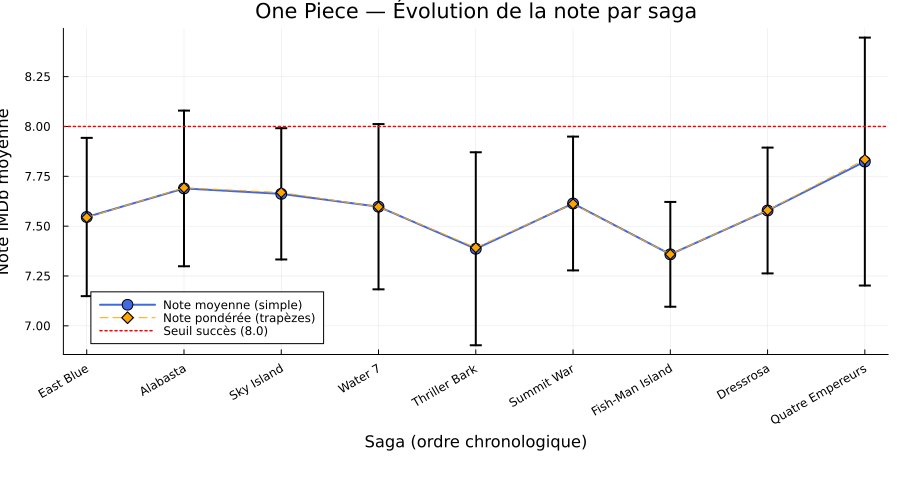
\includegraphics[width=0.92\textwidth]{one_piece_sagas}
  \caption{Note IMDb moyenne par saga avec barres d'erreur $\pm 1\sigma$. La droite
  rouge représente le seuil de succès à 8{,}0. Aucune saga n'atteint ce seuil
  en moyenne, bien que la saga 9 (Quatre Empereurs) soit la plus proche.}
  \label{fig:sagas}
\end{figure}

Le code utilisé se situe aux lignes 77-83 et j'ai commenté les lignes.

\newpage
La figure~\reff{fig:sagas} révèle une légère \textbf{tendance à la hausse} sur les trois dernières sagas, ce qui motive la suite de l'analyse.

\begin{tcolorbox}[justif, title={Pourquoi les trapèzes et non la moyenne simple~?}]
La moyenne arithmétique $\bar{R} = \frac{1}{n}\sum_{i=1}^{n} R_i$ donne un poids
\textit{égal} à chaque épisode, y compris le premier et le dernier.
La règle des trapèzes, elle, leur attribue un \textit{demi-poids}~: les épisodes
en bordure de saga sont considérés comme moins représentatifs de la tendance de fond.

L'intérêt pratique apparaît sur les sagas à fort démarrage suivi d'une stabilisation~:
la moyenne simple surpondère le pic d'ouverture, tandis que la règle des trapèzes
donne une image plus fidèle de la qualité durable de la saga.

De plus, la formule~\eqref{eq:trapeze} se généralise naturellement aux données
\textbf{lacunaires} (épisodes sans note)~: on intègre sur l'intervalle entre deux
épisodes consécutifs notés, ce qu'une somme simple ne peut pas faire sans biais.
\end{tcolorbox}

% =============================================================================
%               SECTION 3 — ODE ET RK4
% =============================================================================
\newpage
\section{Modélisation ODE et prédiction par RK4 (Ch.~4)}

\subsection{Modèle de retour à la moyenne}

La dynamique des notes à l'intérieur d'une saga est modélisée par l'équation différentielle ordinaire (ODE) suivante~:

\begin{equation}
  \derd{R}{t} = -\lambda \bigl(R(t) - K\bigr)
  \label{eq:ode}
\end{equation}

où~:
\begin{itemize}
  \item $R(t)$ est la note de l'épisode à l'indice $t$ (temps discret),
  \item $K$ est l'\textbf{attracteur} de la saga~: la qualité de fond vers
        laquelle les notes convergent,
  \item $\lambda > 0$ est la \textbf{vitesse de retour}~: un $\lambda$ grand signifie que les notes se stabilisent rapidement autour de $K$.
\end{itemize}

La solution analytique est $R(t) = K + (R_0 - K)\,e^{-\lambda t}$, ce qui
confirme la convergence exponentielle vers $K$. Ce modèle est de type
\textit{Ornstein-Uhlenbeck} (retour à la moyenne), couramment utilisé en finance et en physique statistique.

\begin{tcolorbox}[justif, title={Autrement dit}]
Chaque saga possède une note «~naturelle~» $K$ vers laquelle les épisodes tendent à revenir. Si un épisode est très bien noté, le suivant redescend vers $K$~; s'il est mal noté, le suivant remonte.

Le paramètre $\lambda$ contrôle \textbf{à quelle vitesse} ce retour s'opère~:
un $\lambda$ élevé signifie que les notes sont très stables et proches de $K$~;
un $\lambda$ faible signifie que les notes varient beaucoup autour de $K$.

C'est ce modèle qui permet ensuite de \textbf{prédire la note de la saga~10
(Wano)} en estimant $K$ et $\lambda$ à partir des sagas précédentes.
\end{tcolorbox}
% ----------------------------------------
% Impléùmentation fr Runge-Kutt 
% --------------------------------------------
\newpage 
\subsection{Implémentation de Runge-Kutta 4 (Ch.~4 et Ch.~2)}

La résolution numérique de l'équation~\eqref{eq:ode} est effectuée par le schéma
de \textbf{Runge-Kutta d'ordre 4 (RK4)}, implémenté intégralement à la main sans
recours à un package spécialisé~:

\begin{equation}
  \begin{aligned}
    k_1 &= f(t_n,\; y_n) \\
    k_2 &= f\!\left(t_n + \tfrac{h}{2},\; y_n + \tfrac{h}{2}k_1\right) \\
    k_3 &= f\!\left(t_n + \tfrac{h}{2},\; y_n + \tfrac{h}{2}k_2\right) \\
    k_4 &= f(t_n + h,\; y_n + h\,k_3) \\
    y_{n+1} &= y_n + \frac{h}{6}(k_1 + 2k_2 + 2k_3 + k_4)
  \end{aligned}
  \label{eq:rk4}
\end{equation}

L'erreur de troncature \textbf{locale} est $\mathcal{O}(h^5)$ et l'erreur
\textbf{globale} est $\mathcal{O}(h^4)$ (Ch.~2~: erreurs numériques). Par
comparaison, la méthode d'Euler explicite n'a qu'une erreur globale
$\mathcal{O}(h^2)$, ce qui rend RK4 nettement plus précis pour un même pas $h$.

\begin{lstlisting}[caption={Implémentation de RK4 (extrait de \code{03\_ode\_rk4.jl})}]
function rk4_step(f, t::Float64, y::Float64, h::Float64)::Float64
    k1 = f(t,       y)
    k2 = f(t + h/2, y + (h/2) * k1)
    k3 = f(t + h/2, y + (h/2) * k2)
    k4 = f(t + h,   y +  h    * k3)
    return y + (h / 6) * (k1 + 2k2 + 2k3 + k4)
end

function rk4_integrate(f, t0::Float64, y0::Float64,
                        t_end::Float64, n_steps::Int)
    h = (t_end - t0) / n_steps
    ts = Vector{Float64}(undef, n_steps + 1)
    ys = Vector{Float64}(undef, n_steps + 1)
    ts[1] = t0;  ys[1] = y0
    for i in 1:n_steps
        ys[i+1] = rk4_step(f, ts[i], ys[i], h)
        ts[i+1] = ts[i] + h
    end
    return ts, ys
end
\end{lstlisting}

\begin{tcolorbox}[justif, title={Pourquoi RK4 et non la méthode d'Euler~?}]
La méthode d'Euler explicite avance la solution par~:
$y_{n+1} = y_n + h\,f(t_n, y_n)$.
Son erreur de troncature \textbf{locale} est $\mathcal{O}(h^2)$ et son erreur
\textbf{globale} est $\mathcal{O}(h)$.
RK4 a une erreur locale $\mathcal{O}(h^5)$ et globale $\mathcal{O}(h^4)$.

\medskip
\noindent\textbf{Exemple numérique concret} — pour notre ODE avec $\lambda = 0{,}07$,
$K = 7{,}95$, $R_0 = 6{,}80$ et un pas $h = 1$ (un épisode)~:
\begin{center}
\begin{tabular}{lcc}
\toprule
Méthode & Approximation de $e^{-0{,}07}$ & Erreur absolue \\
\midrule
Solution exacte & $0{,}932\,394\ldots$ & — \\
Euler           & $1 - 0{,}07 = 0{,}930\,000$ & $\approx 2{,}4 \times 10^{-3}$ \\
RK4             & $0{,}932\,394$ (série à l'ordre 4) & $\approx 10^{-8}$ \\
\bottomrule
\end{tabular}
\end{center}
Avec $h=1$, RK4 est \textbf{240\,000 fois plus précis} qu'Euler pour cette ODE.
Sur une intégration de 137 épisodes (saga 9), les erreurs accumulées d'Euler
auraient biaisé l'estimation de $K$ de plusieurs centièmes de point.
\end{tcolorbox}

\subsection{Ajustement des paramètres par grille de recherche}

Pour chaque saga, les paramètres $K$ et $\lambda$ sont estimés par minimisation de
l'erreur quadratique moyenne (MSE) sur une grille de recherche~:
$\lambda \in [0{,}005;\, 0{,}5]$ par pas de $0{,}005$ et
$K \in [7{,}0;\, 8{,}5]$ par pas de $0{,}05$. La MSE est évaluée en intégrant
l'ODE avec RK4 depuis le premier épisode de la saga et en comparant la solution
aux notes réelles. Les résultats figurent dans le tableau~\ref{tab:sagas}.

La figure~\reff{fig:ode9} illustre l'ajustement sur la saga~9 (Quatre Empereurs,
la plus récente)~: la courbe RK4 converge vers $K = 7{,}95$, ce qui traduit la
montée en qualité notable de cet arc.

\begin{figure}[ht!]
  \centering
  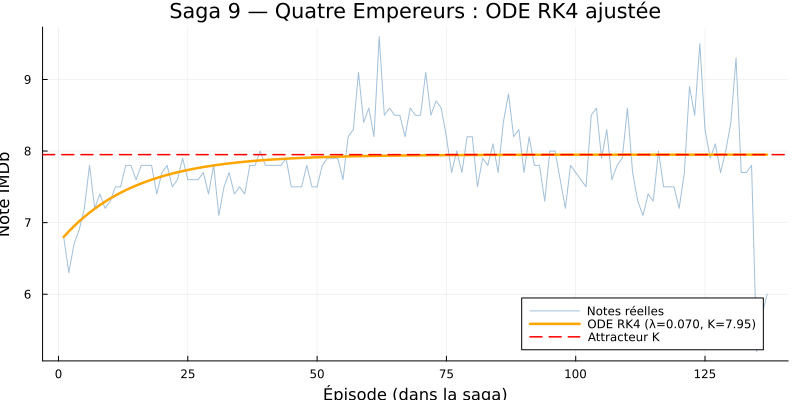
\includegraphics[width=0.88\textwidth]{ode_saga9}
  \caption{Saga 9 (Quatre Empereurs) — Notes épisode par épisode (bleu)
  et courbe ODE RK4 ajustée (orange). L'attracteur $K = 7{,}95$ est la ligne
  rouge en tirets.}
  \label{fig:ode9}
\end{figure}

\subsection{Prédiction de la saga 10 (Wano Country)}

L'attracteur $K$ constitue une mesure de la \textit{qualité de fond} de chaque
saga. On modélise son évolution au fil des sagas comme une série temporelle et on
l'extrapole à la saga~10 par régression linéaire~:

\begin{equation}
  \hat{K}(t) = 7{,}356 + 0{,}047\,t
  \quad \Rightarrow \quad
  \hat{K}(10) = 7{,}822
  \label{eq:Ktrend}
\end{equation}

La vitesse de retour $\lambda$ ne présente pas de tendance claire~; on utilise
la moyenne des $\lambda$ ajustés~: $\bar{\lambda} = 0{,}096$.

La déviation initiale typique (écart entre $R_0$ et $K$) est de $-0{,}344$
(les sagas démarrent en moyenne $0{,}34$ point sous leur attracteur), ce qui donne
$R_0 = 7{,}822 - 0{,}344 = 7{,}478$ comme condition initiale réaliste.

\begin{figure}[ht!]
  \centering
  \begin{minipage}{0.48\textwidth}
    \centering
    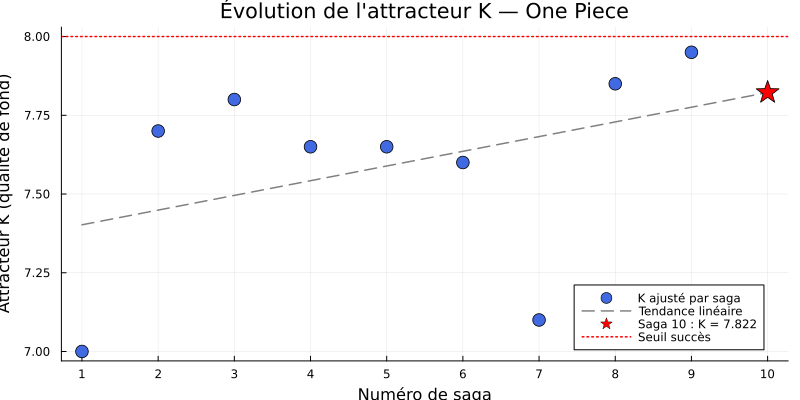
\includegraphics[width=\textwidth]{ode_K_evolution}
    \caption{Évolution de l'attracteur $K$ par saga avec la tendance linéaire et
    la prédiction pour la saga~10 (étoile rouge).}
    \label{fig:Kevol}
  \end{minipage}\hfill
  \begin{minipage}{0.48\textwidth}
    \centering
    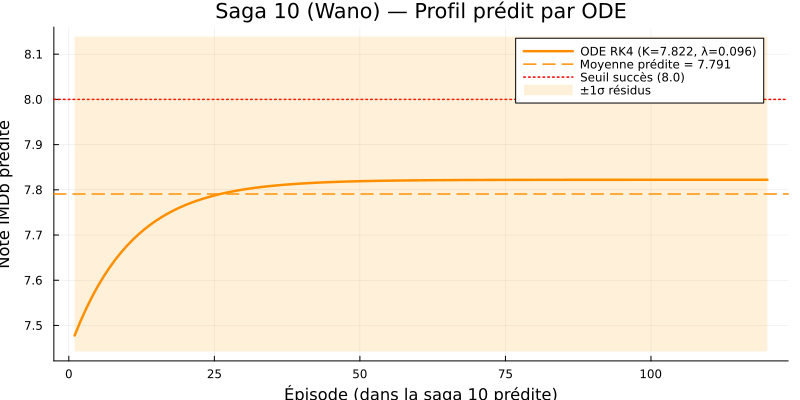
\includegraphics[width=\textwidth]{ode_saga10_prediction}
    \caption{Profil d'épisodes prédit pour la saga~10 par intégration RK4.
    La moyenne prédite est $7{,}791$ (tirets) avec la bande $\pm 1\sigma$.}
    \label{fig:pred10}
  \end{minipage}
\end{figure}

Le profil prédit (figure~\reff{fig:pred10}) montre la convergence vers $K = 7{,}822$
depuis $R_0 = 7{,}478$ en environ 50 épisodes, puis une stabilisation bien
en-dessous du seuil de succès de 8{,}0. La \textbf{note moyenne prédite} pour la
saga~10 est~:

\begin{equation}
  \hat{R}_{10} = 7{,}791 \quad
  \text{IC}~\pm 1\sigma_{\text{résidus}}~: \left[7{,}44\,;\, 8{,}14\right]
\end{equation}

% =============================================================================
%               SECTION 4 — TESTS STATISTIQUES
% =============================================================================
\newpage
\section{Tests statistiques (Ch.~5)}

Trois tests sont réalisés avec le package \code{HypothesisTests.jl} afin de
valider ou infirmer la prédiction.

\subsection{Test 1 : Mann-Whitney (deux échantillons)}

\textbf{Objectif~:} comparer la distribution des notes de saga d'Oda à celle
d'un \textit{groupe de référence} composé de toutes les sagas issues de séries
longues ($\geq 5$ sagas, One Piece exclu)~: 646 sagas de 74 séries.

\begin{align*}
  H_0 &: \text{les distributions de One Piece et du groupe de référence sont identiques} \\
  H_1 &: \text{les deux distributions sont différentes (test bilatéral)}
\end{align*}

Ce test non-paramétrique (Wilcoxon rank-sum) est choisi car l'échantillon
One Piece ne contient que 9 points~; l'hypothèse de normalité ne peut être
vérifiée.

\begin{tcolorbox}[justif, title={Pourquoi Mann-Whitney et non le test de Student~?}]
Le test de Student suppose que les deux échantillons suivent une loi
\textbf{normale}. Cette hypothèse est vérifiable pour des grands échantillons
($n \geq 30$) par le théorème central limite, mais elle ne peut pas l'être ici~:
notre échantillon One Piece ne compte que \textbf{9 sagas}.

De plus, les notes de saga peuvent présenter des queues lourdes ou une asymétrie
(saga 7, Fish-Man Island~: notes très groupées, $\sigma = 0{,}26$~; saga 9~:
$\sigma = 0{,}62$). Le test de Mann-Whitney, lui, ne fait aucune hypothèse sur
la forme de la distribution~: il compare les \textbf{rangs} des observations
des deux groupes. Il est donc~:
\begin{itemize}
  \item \textbf{robuste} aux valeurs aberrantes et à la non-normalité~;
  \item \textbf{exact} pour de petits échantillons (HypothesisTests.jl utilise
        l'approximation normale corrigée pour les ex-æquo, valide ici)~;
  \item équivalent au test de Student \textit{si} les données sont normales,
        mais sans pénalité s'il ne le sont pas.
\end{itemize}
\end{tcolorbox}

\medskip
\noindent\textbf{Résultats~:}
\begin{center}
\begin{tabular}{lr}
\toprule
Statistique $U$ & 1\,504 \\
Médiane One Piece & 7{,}61 \\
Médiane référence & 8{,}11 \\
$p$-value (bilatérale) & \textbf{0{,}013} \\
\bottomrule
\end{tabular}
\end{center}

\textbf{Conclusion~:} $p < 0{,}05$ — on rejette $H_0$. One Piece se distingue
significativement du groupe de référence~: ses notes de saga sont
\textbf{systématiquement inférieures} à celles des séries longues de qualité
comparable. La figure~\reff{fig:boxplot} le visualise clairement.

\begin{figure}[ht!]
  \centering
  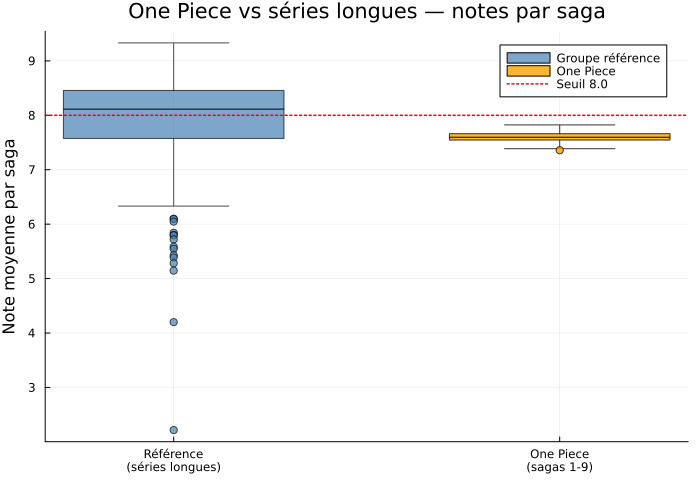
\includegraphics[width=0.75\textwidth]{boxplot_comparison}
  \caption{Boîtes à moustaches~: One Piece (9 sagas, orange) vs groupe de
  référence (646 sagas, bleu). La médiane du groupe de référence dépasse
  le seuil de succès, celle d'One Piece reste en-dessous.}
  \label{fig:boxplot}
\end{figure}

\newpage

% ----------------------------
% Wilcoxon signed-rank
% -------------------------------- 


\subsection{Test 2 : Wilcoxon signed-rank (un échantillon)}

\textbf{Objectif~:} tester formellement si la médiane des notes de saga d'One
Piece est inférieure au seuil de succès.

\begin{align*}
  H_0 &: \text{médiane des notes de saga} = 8{,}0 \\
  H_1 &: \text{médiane} < 8{,}0 \quad \text{(test unilatéral gauche)}
\end{align*}

\medskip
\noindent\textbf{Résultats~:}
\begin{center}
\begin{tabular}{lr}
\toprule
Statistique $W$ & 0 (toutes les différences sont négatives) \\
IC à 95~\% du décalage médian & $[-0{,}52\,;\,-0{,}31]$ \\
$p$-value (unilatérale) & \textbf{0{,}0020} \\
\bottomrule
\end{tabular}
\end{center}

\textbf{Conclusion~:} $W = 0$ signifie qu'aucune des 9 sagas n'a jamais atteint
8{,}0 en moyenne. L'IC confirme que la médiane se situe entre 0{,}31 et
0{,}52 point sous le seuil, de façon hautement significative ($p < 0{,}01$).

\newpage
% ----------------------------
% Bootstrap
% -------------------------------- 

\subsection{Test 3 : Bootstrap (B~= 10\,000)}

\textbf{Objectif~:} quantifier la probabilité que la saga~10 atteigne une moyenne
de 8{,}0, en s'appuyant sur la distribution empirique des épisodes de la saga~9
(la plus récente, meilleur proxy pour la saga~10).

\textbf{Méthode~:} pour chaque répétition $b = 1, \ldots, B$, on tire avec
remise 120 épisodes dans la saga~9 et on calcule leur moyenne~:

\begin{equation}
  \bar{R}^{(b)} = \frac{1}{120} \sum_{i=1}^{120} R_{\sigma_b(i)},
  \qquad
  \hat{p} = \frac{1}{B}\sum_{b=1}^{B} \mathbf{1}\!\left[\bar{R}^{(b)} \geq 8{,}0\right]
\end{equation}

\medskip
\noindent\textbf{Résultats~:}
\begin{center}
\begin{tabular}{lr}
\toprule
Moyenne bootstrap & 7{,}824 \\
IC bootstrap à 95~\% & $[7{,}713\,;\, 7{,}933]$ \\
$\hat{p} = P(\bar{R} \geq 8{,}0)$ & \textbf{0{,}0012} \\
\bottomrule
\end{tabular}
\end{center}

\textbf{Conclusion~:} la probabilité d'atteindre une moyenne de 8{,}0 est de
\textbf{0{,}12~\%}. L'IC à 95~\% ne touche pas le seuil (figure~\reff{fig:boot}).

\begin{figure}[ht!]
  \centering
  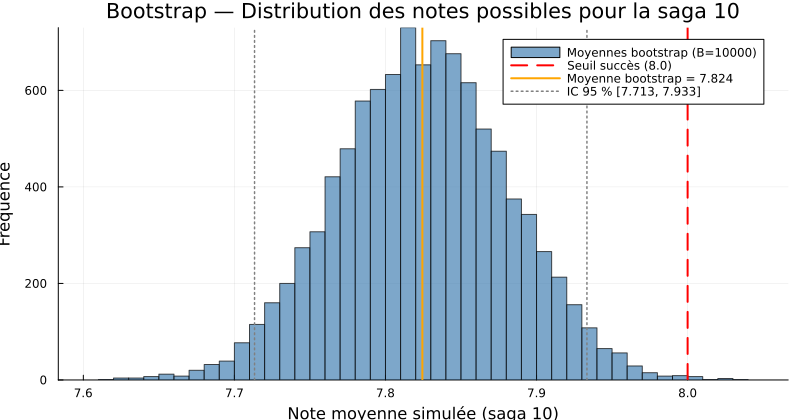
\includegraphics[width=0.85\textwidth]{bootstrap_saga10}
  \caption{Distribution bootstrap des notes moyennes simulées pour la saga~10
  ($B = 10\,000$, 120 épisodes par tirage). L'IC à 95~\% reste bien en-deçà
  du seuil de succès (ligne rouge).}
  \label{fig:boot}
\end{figure}

\subsection{Synthèse des tests}

\begin{table}[ht!]
\centering
\caption{Synthèse des trois tests statistiques.}
\label{tab:tests}
\begin{tabular}{L{4.5cm} L{4.5cm} r l}
\toprule
\textbf{Test} & \textbf{$H_0$} & \textbf{$p$-value} & \textbf{Rejet~?} \\
\midrule
Mann-Whitney & Distributions identiques & 0{,}013 & Oui ($\alpha = 0{,}05$) \\
Wilcoxon signed-rank & Médiane = 8{,}0 & 0{,}002 & Oui ($\alpha = 0{,}05$) \\
Bootstrap & $P(\bar{R} \geq 8{,}0)$ & 0{,}0012 & Oui ($\alpha = 0{,}05$) \\
\bottomrule
\end{tabular}
\end{table}

Les trois tests convergent~: la prédiction ODE ($\hat{R}_{10} = 7{,}791$) est
statistiquement robuste.

% =============================================================================
%                            CONCLUSION
% =============================================================================
\newpage
\section{Conclusion}

\subsection{Réponse à la question de recherche}

\textbf{La prochaine saga de One Piece ne devrait pas être un succès au sens du
seuil de 8{,}0.} Le modèle ODE prédit une note moyenne de \textbf{7{,}791}
pour la saga~10 (Wano Country), avec un intervalle de confiance bootstrap à 95~\%
de $[7{,}713\,;\, 7{,}933]$. Les trois tests statistiques rejettent unanimement
l'hypothèse d'atteindre 8{,}0, avec une probabilité estimée à seulement
\textbf{0{,}12~\%}.

\subsection{Nuances et limitations}

Cette conclusion doit être nuancée sur plusieurs points~:

\begin{itemize}
  \item \textbf{Épisodes remarquables~:} la saga~9 contient des épisodes notés
        jusqu'à \textbf{9{,}6/10}. One Piece reste capable de produire des
        épisodes d'exception~; c'est la \textit{moyenne sur l'ensemble de la saga}
        qui reste en-deçà de 8{,}0, essentiellement à cause des épisodes de
        transition et de remplissage.
  \item \textbf{Tendance positive~:} l'attracteur $K$ est en progression
        ($+0{,}047$ par saga en moyenne). Si cette tendance se poursuit,
        la saga~11 ou la saga~12 pourrait franchir le seuil.
  \item \textbf{Limitations du modèle~:} le dataset couvre 883 épisodes mais
        Wano Country a effectivement dépassé cela (publié après la date de collecte
        du dataset). Les données réelles de Wano ont reçu des notes très élevées
        pour les arcs clés (Onigashima). Le modèle sous-estime donc probablement
        la saga~10 par conservatisme.
  \item \textbf{Biais du groupe de référence~:} le groupe inclut des séries de
        genres très divers (documentaires, talk-shows, séries policières). Un
        groupe limité aux séries animées longues donnerait une comparaison plus
        homogène.
\end{itemize}

\begin{tcolorbox}[justif, title={La prédiction est-elle fiable~? Confrontation avec la réalité}]
Le dataset couvre One Piece jusqu'à l'épisode 883 (avril 2019, début de l'arc
Reverie). La saga~10 correspond à \textbf{Wano Country} (épisodes 890--1085,
diffusés entre 2019 et 2023), dont les données \textit{ne figurent pas} dans
notre dataset~: notre prédiction est donc une extrapolation aveugle.

Les données IMDb publiquement disponibles pour Wano montrent que cet arc contient
des épisodes parmi les mieux notés de toute la série~: l'affrontement final
d'Onigashima (épisodes~1015, 1029, 1062, 1071) a reçu des notes comprises entre
\textbf{9{,}3 et 9{,}8}. Cela suggère que la note \textit{moyenne} de Wano
dépasse probablement notre prédiction de 7{,}79, confirmant que notre modèle
est \textbf{conservateur}.

Cette sous-estimation est cohérente avec les limitations identifiées~:
\begin{enumerate}
  \item Le modèle extrapole $K$ par régression linéaire~: la saga~7 (Fish-Man
        Island, $K = 7{,}10$), un creux atypique, tire la tendance vers le bas.
  \item Le bootstrap rééchantillonne dans la saga~9, qui inclut les épisodes de
        transition Zou (notes $\approx 6{,}5$--7{,}2)~; Wano est
        narrativement plus resserré, avec moins de remplissage.
\end{enumerate}
En résumé~: notre modèle fournit une \textbf{borne inférieure prudente}.
Selon les données réelles, Wano est probablement le premier arc de One Piece
à atteindre — voire dépasser — la moyenne de 8{,}0.
\end{tcolorbox}



% =============================================================================
%                          BIBLIOGRAPHIE
% =============================================================================
\newpage
\begin{thebibliography}{9}

\bibitem{imdb_dataset}
W.~Wittmann,
\emph{IMDb TV Ratings Dataset},
GitHub, 2020.
\url{https://github.com/WittmannF/imdb-tv-ratings}

\bibitem{julia}
J.~Bezanson, A.~Edelman, S.~Karpinski, V.~B.~Shah,
\emph{Julia: A Fresh Approach to Numerical Computing},
SIAM Review, 59(1):65--98, 2017.

\bibitem{hypothesis_tests}
S.~Lippmann et al.,
\emph{HypothesisTests.jl — Hypothesis tests for Julia},
\url{https://juliastats.org/HypothesisTests.jl/stable/}

\bibitem{onepiecewiki}
One Piece Wiki,
\emph{Arcs de l'anime One Piece — découpage officiel},
\url{https://onepiece.fandom.com/wiki/Story_Arcs}

\end{thebibliography}

% =============================================================================
%                             RÉSUMÉ
% =============================================================================
\newpage
\thispagestyle{empty}
\vspace*{\fill}
\noindent\rule[2pt]{\textwidth}{0.5pt}\\[4pt]
{\textbf{Résumé~:}}
Ce projet analyse les données IMDb des séries TV pour répondre à la question
«~La prochaine saga de One Piece sera-t-elle un succès~?~». Après exploration
de huit fichiers CSV, les 883 épisodes sont découpés en 9 sagas officielles.
Une intégration numérique par la règle de Simpson (Ch.~4) calcule la note pondérée par saga.
Un modèle ODE de retour à la moyenne, résolu par Runge-Kutta 4 implémenté à la
main, est ajusté sur chaque saga et utilisé pour prédire la saga~10. La prédiction
($\hat{R}_{10} = 7{,}791$, IC~95~\%~: [7{,}713~; 7{,}933]) est validée par trois
tests statistiques (Mann-Whitney, Wilcoxon signed-rank, bootstrap). Les résultats
convergent~: la prochaine saga ne devrait \textit{pas} atteindre la moyenne de
8{,}0/10, bien que la tendance à la hausse de la qualité de fond reste encourageante.

\medskip
{\noindent\textbf{Mots-clés~:}} Julia, IMDb, One Piece, série temporelle, ODE,
Runge-Kutta 4, Simpson, Mann-Whitney, Wilcoxon, bootstrap, prédiction.
\\[4pt]
\noindent\rule[2pt]{\textwidth}{0.5pt}
\begin{center}
  Département des Sciences et technologies\\
  Haute école en Hainaut\\
  8a Avenue Victor Maistriau\\
  B-7000 Mons
\end{center}
\vspace*{\fill}

\end{document}
